\begin{spacing}{1.5}
    \section{Graph Contraction}\\

    \noindent Graph contraction itself is trivial, but what is needed is a method of contracting the graph while retaining all information about
    the original graph to enable routing points to be re-inserted.

    \vspace{12pt}\subsection{Initial Contraction}
    \noindent The following figure illustrates a non-contracted graph. Consider a process of contraction which starts by removal of the vertex B.

    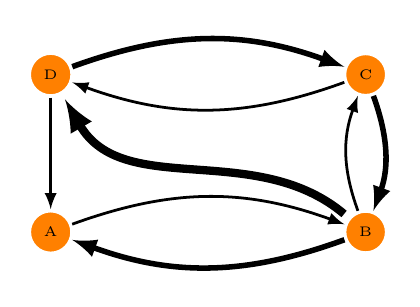
\begin{tikzpicture}[font=\tiny]
    \tikzstyle{node_style} = [draw=white, very thick, circle, fill=orange]
    \tikzstyle{arrow_style1} = [->, black, line width=1, >=latex]
    \tikzstyle{arrow_style2} = [->, black, line width=2, >=latex]
    \tikzstyle{arrow_style3} = [->, black, line width=3, >=latex]
    \tikzstyle{edge_style2} = [lightgray, line width=1]


    \node[node_style] (n1) at (0,0) {A};
    \node[node_style] (n2) at (4,0) {B};
    \node[node_style] (n3) at (4,2) {C};
    \node[node_style] (n4) at (0,2) {D};

    \draw[arrow_style1] (n1) edge [bend left=20] (n2);
    \draw[arrow_style2] (n2) edge [bend left=20] (n1);
    \draw[arrow_style1] (n2) edge [bend left=20] (n3);
    \draw[arrow_style2] (n3) edge [bend left=20] (n2);
    \draw[arrow_style1] (n3) edge [bend left=20] (n4);
    \draw[arrow_style2] (n4) edge [bend left=20] (n3);
    \draw[arrow_style1] (n4) edge (n1);
    \draw[arrow_style3, shorten <=2pt, shorten >=2pt] (n2) edge [out=140, in=-60] (n4);
\end{tikzpicture}


    Contraction requires the following maps:

    \begin{enumerate}
        \item{\tt vert2edge}
        \item{\tt old2new} --- A simple map of old-to-new edge numbers
        \item{\tt new2old} --- A map of new edge numbers to structures detailed below
    \end{enumerate}

    Replacing edges 2 \& 3 with a single edge\#8 then gives the following mappings:
    \begin{lstlisting}
        vert2edge(B)     = 8
        old2new(2)       = 8
        old2new(3)       = 8
        new2old(8).verts = [A, B, C]
        new2old(8).edges = [2, 3]
        new2old(8).d     = [d.AB, d.BC]
    \end{lstlisting}
    Removal of vertex B also requires replacing the edges 5 \& 6.  Note that the {\tt new2old} maps have to be constructed such that the {\tt
    in} edge is first inserted, followed by the {\tt out} edge, so in this case, edge\#6 comes before \#5, giving the following mappings:
    \begin{lstlisting}
        vert2edge(B)     = [8, 9]
        old2new(5)       = 9
        old2new(6)       = 9
        new2old(9).verts = [C, B, A]
        new2old(9).edges = [6, 5]
        new2old(9).d     = [d.CB, d.BA]
    \end{lstlisting}

    That reduces the graph to:

    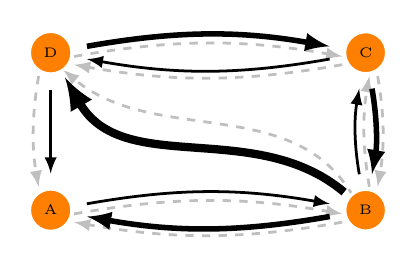
\begin{tikzpicture}[font=\tiny, >=latex, shorten >=5pt, shorten <=5pt]
    \tikzstyle{nonode} = []
    \tikzstyle{node_style} = [draw=white, very thick, circle, fill=orange]
    \tikzstyle{black_arrow1} = [->, black, line width=1]
    \tikzstyle{black_arrow2} = [->, black, line width=2]
    \tikzstyle{black_arrow3} = [->, black, line width=3]
    \tikzstyle{grey_arrow} = [->, lightgray, dashed, line width=1]

    \node[nonode] (nAd) at (0,-0.1) {};
    \node[nonode] (nAl) at (-0.1,0) {};
    \node[nonode] (nBd) at (4,-0.1) {};
    \node[nonode] (nBr) at (4.1,0) {};
    \node[nonode] (nCd) at (4,1.9) {};
    \node[nonode] (nCr) at (4.1,2) {};
    \node[nonode] (nDd) at (0,1.9) {};
    \node[nonode] (nDl) at (-0.1,2) {};

    \draw[grey_arrow] (nAd) edge [bend left=10] (nBd);
    \draw[grey_arrow] (nBd) edge [bend left=10] (nAd);
    \draw[grey_arrow] (nBr) edge [bend left=10] (nCr);
    \draw[grey_arrow] (nCr) edge [bend left=10] (nBr);
    \draw[grey_arrow] (nCd) edge [bend left=10] (nDd);
    \draw[grey_arrow] (nDd) edge [bend left=10] (nCd);
    \draw[grey_arrow] (nDl) edge [bend right=10] (nAl);
    \draw[grey_arrow] (nBd) edge [out=120, in=-40] (nDl);

    \node[node_style] (nA) at (0,0) {A};
    \node[node_style] (nB) at (4,0) {B};
    \node[node_style] (nC) at (4,2) {C};
    \node[node_style] (nD) at (0,2) {D};

    \draw[black_arrow1] (nA) edge [bend left=10] (nB);
    \draw[black_arrow2] (nB) edge [bend left=10] (nA);
    \draw[black_arrow1] (nB) edge [bend left=10] (nC);
    \draw[black_arrow2] (nC) edge [bend left=10] (nB);
    \draw[black_arrow1] (nC) edge [bend left=10] (nD);
    \draw[black_arrow2] (nD) edge [bend left=10] (nC);
    \draw[black_arrow1] (nD) edge (nA);

    \draw[black_arrow3, shorten <=2pt, shorten >=2pt] (nB) edge [out=140, in=-60] (nD);
\end{tikzpicture}


    The vertex C can then be removed by first replacing the edges 8 \& 4 through the mappings:
    \begin{lstlisting}
        vert2edge(C)      = 10
        old2new(8)        = 10
        old2new(4)        = 10
        new2old(10).verts = [A, B, C, D]
        new2old(10).edges = [2, 3, 4]
        new2old(10).d     = [d.AB, d.BC, d.CD]
    \end{lstlisting}
    Note that {\tt new2old().edges} contains only those edge numbers present in the original graph. Thus {\tt new2old(10).edges} does *not* have
    edge\#8. This is ensured simply by only inserting in these {\tt new2old().edges} lists those edges not actually found in the map itself.
    Because {\tt new2old.find(8) != new2old.end()}, that edge is not inserted.

    Replacing edges 7 \& 9 with edge\#11 requires first identifying that vertex D connects to C, and that C is the {\it first} item of the {\tt
    new2old(9).verts}. New values are therefore pushed onto the front to give,
    \begin{lstlisting}
        vert2edge(C)      = [10, 11]
        old2new(9)        = 11
        old2new(7)        = 11
        new2old(11).verts = [D, C, B, A]
        new2old(11).edges = [7, 6, 5]
        new2old(11).d     = [d.DC, d.BC, d.BA]
    \end{lstlisting}

    \pagebreak
    This finally gives the desired contraction.

    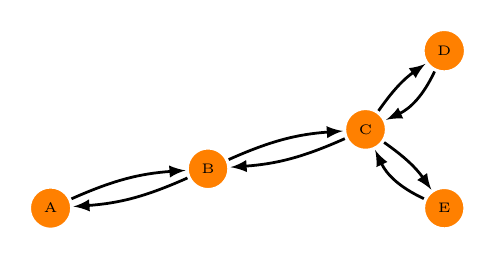
\begin{tikzpicture}[font=\tiny]
    \tikzstyle{node_style} = [draw=white, very thick, circle, fill=orange]
    \tikzstyle{arrow_style1} = [->, black, line width=1, >=latex]

    \node[node_style] (n1) at (0,0) {A};
    \node[node_style] (n2) at (2,0.5) {B};
    \node[node_style] (n3) at (4,1) {C};
    \node[node_style] (n4) at (5,2) {D};
    \node[node_style] (n5) at (5,0) {E};

    \draw[arrow_style1] (n1) edge [bend left=10] (n2);
    \draw[arrow_style1] (n2) edge [bend left=10] (n1);
    \draw[arrow_style1] (n2) edge [bend left=10] (n3);
    \draw[arrow_style1] (n3) edge [bend left=10] (n2);
    \draw[arrow_style1] (n3) edge [bend left=10] (n4);
    \draw[arrow_style1] (n4) edge [bend left=20] (n3);
    \draw[arrow_style1] (n3) edge [bend left=10] (n5);
    \draw[arrow_style1] (n5) edge [bend left=20] (n3);
    %\draw[arrow_style3, shorten <=2pt, shorten >=2pt] (n2) edge [out=140, in=-60] (n4);
\end{tikzpicture}


    The resultant maps are:
    \begin{lstlisting}
        vert2edge(B)      = [8, 9]
        vert2edge(C)      = [10, 11],

        old2new(2)        = 8
        old2new(3)        = 8
        old2new(5)        = 9
        old2new(6)        = 9
        old2new(8)        = 10
        old2new(4)        = 10
        old2new(9)        = 11
        old2new(7)        = 11,

        new2old(8).verts  = [A, B, C]
        new2old(8).edges  = [2, 3]
        new2old(8).d      = [d.AB, d.BC]
        new2old(9).verts  = [C, B, A]
        new2old(9).edges  = [6, 5]
        new2old(9).d      = [d.CB, d.BA]
        new2old(10).verts = [A, B, C, D]
        new2old(10).edges = [2, 3, 4]
        new2old(10).d     = [d.AB, d.BC, d.CD]
        new2old(11).verts = [D, C, B, A]
        new2old(11).edges = [7, 6, 5]
        new2old(11).d     = [d.DC, d.BC, d.BA]
    \end{lstlisting}

    \pagebreak
    \vspace{12pt}\subsection{Graph reconstruction}

    \noindent The maps can then be used to reconstruct a graph. Consider the re-insertion of Vertex {\tt B}. First
    \begin{lstlisting}
        vert2edge(B) = [8, 9]
    \end{lstlisting}
    Then trace new edges for both of those vertices:
    \begin{lstlisting}
        old2new(8)   = 10
        old2new(10) = old2new.end()
        old2new(9)   = 11
        old2new(11) = old2new.end()
    \end{lstlisting}
    so the information we need to re-insert {\tt B} is in the new edges {\tt 10} and {\tt 11}:
    \begin{lstlisting}
        new2old(10).verts = [A, B, C, D]
        new2old(10).edges = [2, 3, 4]
        new2old(10).d     = [d.AB, d.BC, d.CD]
        new2old(11).verts = [D, C, B, A]
        new2old(11).edges = [7, 6, 5]
        new2old(11).d     = [d.DC, d.BC, d.BA]
    \end{lstlisting}
    All that is needed is to trace each {\tt .verts} list until {\tt B} appears, and break the edge to insert a new one. In pseudo-code for
    edge\#10:
    \begin{lstlisting}
        newedge1.from = new2old(10).verts(0) # = A
        newedge1.to   = B
        newedge2.from = B
        newedge2.to   = new2old(10).verts.end() # = D
        d = 0
        for (v in new2old(10).verts):
            if (v == B):
                newedge1.d = d
                d = 0
        newedge2.d = d
        edges_to_remove.push_back (10)
        edges.emplace (12, newedge1) # 12 is number of new edge
        edges.emplace (13, newedge2)
    \end{lstlisting}
    And same for edge\#11.  Consider then the slightly different case of re-inserting Vertex {\tt C}.
    \begin{lstlisting}
        vert2edge(C) = [10, 11]
        old2new(10)  = old2new.end()
        old2new(11)  = old2new.end()
    \end{lstlisting}
    leading this time straight to edges 10 and 11 as the ones to break. For edge\#11:
    \pagebreak
    \begin{lstlisting}
        newedge1.from = new2old(11).verts(0) # = C
        newedge1.to   = C
        newedge2.from = C
        newedge2.to   = new2old(11).verts.end() # = A
        d = 0
        for (v in new2old(10).verts):
            if (v == C):
                newedge1.d = d
                d = 0
        newedge2.d = d
        edges_to_remove.push_back (10)
    \end{lstlisting}
    That works for single insertions, but it will fail if two vertices need to be re-inserted on the same edge. For that to work, the maps need
    to be updated to reflect vertex re-insertions.

    \vspace{12pt}\subsection{Updating Maps}

    \noindent Updating maps requires extending the pseudo-code above. Consider again the re-insertion of Vertex {\tt B}
    \begin{lstlisting}
        newedge1.from = new2old(10).verts(0) # = A
        newedge1.to   = B
        newedge2.from = B
        newedge2.to   = new2old(10).verts.end() # = D
        new2old(12).verts[0] = newedge1.from
        new2old(13).verts[0] = newedge2.from
        d = 0
        for (v in new2old(10).verts):
            vert2edge(v).remove(10) # will remove vert2edge(C) = 10
            if (v <= B)
                vert2edge(v).insert(12) # vert2edge(B)=12
                new2old(12).verts.push_back(v)
                new2old(12).edges.push_back(e)
                new2old(12).d.push_back(d)
            if (v >= B)
                vert2edge(v).insert(13) # vert2edge(C)=13
                new2old(13).verts.push_back(v)
                new2old(13).edges.push_back(e)
                new2old(13).d.push_back(d)
            if (v == B):
                newedge1.d = d
                d = 0
        newedge2.d = d
        edges_to_remove.push_back (10)
        edges.emplace (12, newedge1)
        edges.emplace (13, newedge2)
        vert2edge(B) = [12, 13]
    \end{lstlisting}
    This will yield the following maps
    \begin{lstlisting}
        vert2edge(B)      = [12, 13]
        vert2edge(C)      = [13, 11]

        new2old(8).verts  = [A, B, C]
        new2old(8).edges  = [2, 3]
        new2old(8).d      = [d.AB, d.BC]
        new2old(9).verts  = [C, B, A]
        new2old(9).edges  = [6, 5]
        new2old(9).d      = [d.CB, d.BA]
        new2old(10).verts = [A, B, C, D]
        new2old(10).edges = [2, 3, 4]
        new2old(10).d     = [d.AB, d.BC, d.CD]
        new2old(11).verts = [D, C, B, A]
        new2old(11).edges = [7, 6, 5]
        new2old(11).d     = [d.DC, d.CB, d.BA]
        new2old(12).verts = [A, B]
        new2old(12).edges = [2]
        new2old(12).d     = [d.AB]
        new2old(13).verts = [B, C, D]
        new2old(13).edges = [3, 4]
        new2old(13).d     = [d.BC, d.CD]
    \end{lstlisting}
    Repeating the same procedure for edge\#11, replacing with new edges \#14-15, will then give,
    \begin{lstlisting}
        vert2edge(B)      = [12, 13, 14, 15]
        vert2edge(C)      = [13, 14]

        new2old(8).verts  = [A, B, C]
        new2old(8).edges  = [2, 3]
        new2old(8).d      = [d.AB, d.BC]
        new2old(9).verts  = [C, B, A]
        new2old(9).edges  = [6, 5]
        new2old(9).d      = [d.CB, d.BA]
        new2old(10).verts = [A, B, C, D]
        new2old(10).edges = [2, 3, 4]
        new2old(10).d     = [d.AB, d.BC, d.CD]
        new2old(11).verts = [D, C, B, A]
        new2old(11).edges = [7, 6, 5]
        new2old(11).d     = [d.DC, d.BC, d.BA]
        new2old(12).verts = [A, B]
        new2old(12).edges = [2]
        new2old(12).d     = [d.AB]
        new2old(13).verts = [B, C, D]
        new2old(13).edges = [3, 4]
        new2old(13).d     = [d.BC, d.CD]
        new2old(14).verts = [D, C, B]
        new2old(14).edges = [7, 6]
        new2old(14).d     = [d.DC, d.CB]
        new2old(15).verts = [B, A]
        new2old(15).edges = [5]
        new2old(15).d     = [d.BA]
    \end{lstlisting}
    Note that the {\tt old2new} maps don't need to be updated here because the {\tt vert2edge} maps are directed straight to the new edges which
    have no entries in {\tt vert2edge}. This allows for subsequent re-insertion of vertex\#C through simply tracing,
    \begin{lstlisting}
        vert2edge(C)      = [13, 14]
        new2old(13).verts = [B, C, D]
        new2old(13).edges = [3, 4]
        new2old(13).d     = [d.BC, d.CD]
        new2old(14).verts = [D, C, B]
        new2old(14).edges = [7, 6]
        new2old(14).d     = [d.DC, d.CB]
    \end{lstlisting}
    And re-inserting accordingly.  Note that edge re-construction could theoretically just replace edges with original numbers in cases where
    {\tt newold().edges} only had one component, but the pseudo-code above requires the {\tt vert2edge} maps to be dynamically updated during
    the loop over {\tt v}, before it would be known whether or not this is the case. It'll thus be easier to simply re-number all new edges
    regardless of whether they duplicated pre-existing ones.


    \pagebreak
    \vspace{12pt}\subsection{Updating Maps}

    \noindent Finally, the maps have to be returned as {\tt RCpp} objects. This is straightforward for {\tt old2new}, which only ever contains
    single values, and also for {\tt vert2edge}, which can simply be flattened out to map each vertex onto corresponding one or more new edges.
    The only non-trivial map is {\tt new2old}, which has {\tt .verts}, {\tt .edges}, and {\tt .d} (and in the full implementation, {\tt .w} as
    well). The {\tt .verts} always have one more entry than all other components, and so can be mapped pair-wise to individual elements of the
    others. These flattened versions thus contain five columns of [{\tt new edge number, vert from, vert to, old edge number, dist}].  The
    flatted version of the preceding final {\tt new2old(13)}, restated here for reference as,
    \begin{lstlisting}
        new2old(13).verts = [B, C, D]
        new2old(13).edges = [3, 4]
        new2old(13).d     = [d.BC, d.CD]
    \end{lstlisting}
    would be,
    \begin{lstlisting}
        new2oldf(0) = [13, B, C, 3, d.BC]
        new2oldf(1) = [13, C, D, 4, d.CD]
    \end{lstlisting}
\end{spacing}

